\section{BBA}

% 2024-06-10-SI_bba
% 2024-06-16-SI_bba_tests
% 2024-06-17-SI_bba


\begin{frame}{BBA}
\vspace{-0.2cm}
{\footnotesize
\begin{itemize}
    \setlength\itemsep{0.5em}
    \item estudos em 2024-06-10, 2024-06-16 e 2024-06-17
    \item BBA do dia 05-10 com resultados estranhos: assinaturas da variação de órbita com delta negativo dos trims dos quads correspondiam distorções distribuídas.
    \item BBAs antes e depois da parada do dia 17: OK. Maior variação no 03M2 (cabo movimentado na parada para acomodar outros cabos da SRFCav)
    \item os problemas do dia 10 não voltaram a acontecer. não entendemos...
\end{itemize}
}
\centering
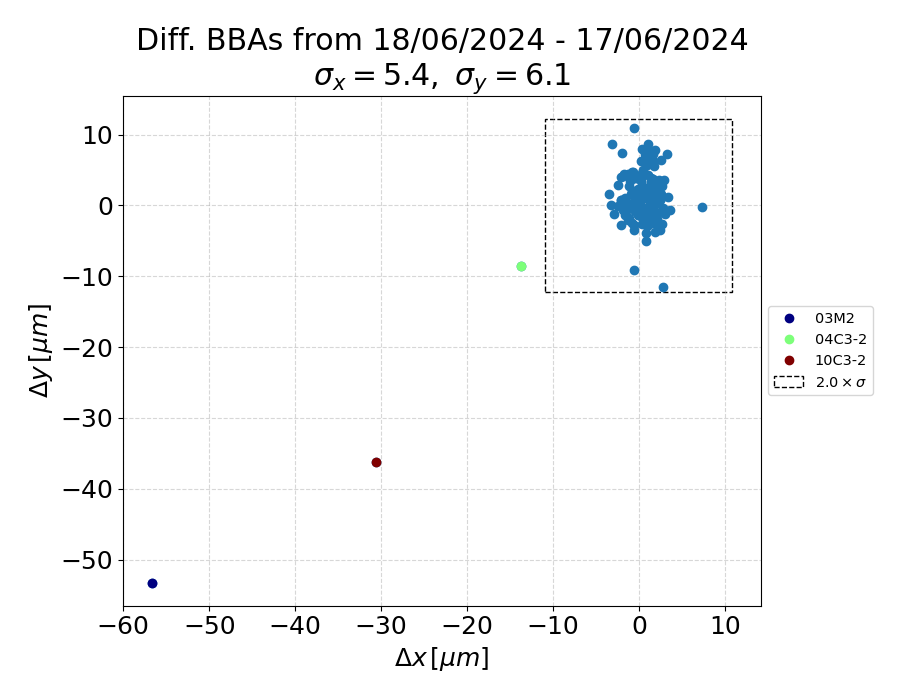
\includegraphics[width=0.4\linewidth]{2024-07-12/figures/diff_to_bba_orb_before_2024_06_17_shutdown.png}
\end{frame}